\documentclass[titlepage,a4paper,12pt]{article}
\usepackage{listings}
\usepackage{amsmath}
\usepackage{amsfonts}
\usepackage{url}
\usepackage[toc,page]{appendix}
\usepackage{algpseudocode}
\usepackage{pgfplots}

\title{The Gravitational N-body System}
\author{Emil Tullstedt}
\date{2016-03-25}

\lstset{
  language=C,
  basicstyle=\footnotesize\ttfamily,
  numbers=left,
  breaklines=true,
  frame=lr,
  captionpos=b,
  showstringspaces=false
}

\begin{document}
\maketitle

\tableofcontents

\newpage
\section{Introduction}
\textit{The gravitational n-body problem} simulates how the gravitational force
affects a number of bodies within a system of particles. By parallelising and
approximating gravitational forces simulations can spend less time calculating
the effects of different gravitational bodies reacting to each other. Efficient
calculations of how particles interact to each other is crucial for astronomics
to be aware of satellites, space debris, asteroids et.c. will affect human life
both short- and long-term.

The simulations described in this report are two-dimensional and rudimentary as
to show the different methods of increasing efficiency rather than constructing
useful simulation data. A video showing a simulation in action can be seen on
YouTube, \url{https://www.youtube.com/watch?v=AH0PfpAryfc} or generated as a
mpeg4-video using the \texttt{plot.py} helper application described in appendix
\ref{sec:plotpy} together with the \texttt{output} file from the 
\texttt{*.debug.out}-versions of the program.

\section{Programs}
\subsection{Na\"{i}ve Sequential Program}
\label{subsec:seq_sq}

The naive sequential program does two things, it calculates how two bodies
affect each other and it uses these calculations to move the bodies. The
simulation uses steps over $dt$ rather than continous calculations.

\subsubsection{Calculating Forces}
\label{subsubsec:calculatingforces}
In order to calculate the forces acting on every particle, for every step
and every particle $i$ the distance $p(ij)$ between that particle and every
other particle $j$ is calculated using Pythagora's Theorem is applied to find
the shortest distance between the two particles.

\begin{equation}
p(ij) = \sqrt{(p(i)_x - p(j)_x)^2 + (p(i)_y - p(j)_y)^2}
\end{equation}

The exponentially diminishing effect of distance $p(ij)$ to the gravitational
force is then applied to Newton's gravitational constant $G = 6.67*10^{-11}$ and
the mass of the two particles using

\begin{equation}
m(ij) = \dfrac{G*m(i)*m(j)}{p(ij)^2}
\end{equation}

The direction of the movement is calculated for the $x$ and $y$ axis 

\begin{align}
d(ij)_x &= p(j)_x - p(i)_x\\
d(ij)_y &= p(j)_y - p(j)_y
\end{align}

Finally, these calculations are applied on the current force in both directions
of the particle $i$

\begin{align}
f(i)_x &= f(i)_x + \dfrac{m(ij) * d(ij)_x}{p(ij)}\\
f(i)_y &= f(i)_y + \dfrac{m(ij) * d(ij)_y}{p(ij)}
\end{align}

Furthermore, as the forces $f(i)_x$ and $f(j)_x$ are each other's opposites
the forces $f(j)_{xy}$ can be calculated with subtraction of the force rather
than addition of it in order to avoid having to calculated both $p(ij)$ and
$p(ji)$ (which are equal), $m(ij)$ and $m(ji)$ (also equal), and $d(ij)$ and
$d(ji)$ (which are opposites).

\begin{align}
f(j)_x &= f(i)_x - \dfrac{m(ij) * d(ij)_x}{p(ij)}\\
f(j)_y &= f(i)_y - \dfrac{m(ij) * d(ij)_y}{p(ij)}
\end{align}

This operation is $O(n^2)$ for $n$ particles.

\subsubsection{Applying Forces}

Applying the forces is an $O(n)$ operation once the calculations in section
\ref{subsubsec:calculatingforces} are applied. For every particle $i$ the
following equation is ran to get the new velocity and position of the particle.

\begin{align}
\delta v(i)_x &= \dfrac{f(i)_x}{m(i)} * dt\\
\delta v(i)_y &= \dfrac{f(i)_y}{m(i)} * dt\\
\delta p(i)_x &= (v(i)_x + \dfrac{\delta v(i)_x}{2}) * dt \\
\delta p(i)_y &= (v(i)_y + \dfrac{\delta v(i)_y}{2}) * dt \\
v(i)_x &= v(i)_x + \delta v(i)_x\\
v(i)_y &= v(i)_y + \delta v(i)_y\\
p(i)_x &= p(i)_x + \delta p(i)_x\\
p(i)_y &= p(i)_y + \delta p(i)_y
\end{align}

And finally resetting the forces in both directions $f(i)$ to $0$.

\subsection{Na\"{i}ve Parallell Program}
\label{subsec:par_sq}
Parallelising the sequential application described in section
\ref{subsec:seq_sq} is primarily a matter of changing the for loops in such a
manner so that every thread will take care of individual particles $i$. In
order to keep the performance gain by applying the forces bi-directionally
the force $f(i)$ is stored as $f(i(t))$ which are then summed together 
$f(i) = f(i(t_0)) + f(i(t_1)) + \cdots + f(i(t_n))$ for $n$ threads before
applying the forces.

A ``barrier'' between the calculation and application of the forces is necessary
to avoid threads from applying unfinished data and corrupting the output. This
barrier was implemented using a shared counter $b(c)$ and a conditional variable
$b(v)$ where a barrier is initialised by setting a value $b(c) \in \mathbb{Z}^+$
for the $c$ threads which must meet at the barrier in order for the conditional
variable $b(v)$ to signal all threads to continue.

\subsection{Barnes-Hut Sequential Program}
\label{subsec:seq_nlg}

The Barnes-Hut approximation of a gravitational n-body system uses the
assumption that any particle far away enough may be calculated as a sum
of the particles in that particle's proximity. This assumption works in the same
way as if someone would answer ``1067'' on the question ``Which year did the 
Battle of Hastings break out?'' that answer would be close to the correct
answer, whereas if someone were to pay their rent one year overdue, their
landlord would probably not be as forgiving as a history teacher might be
about misplacing the Battle of Hastings.

The implementation of the approximation was made with a tree of quadrants where
every quadrant leaf represents $0 \le n \le 5$ particles. If a quadrant leaf
is filled with more than $5$ particles, it would split into four new quadrants
and thus become a quadrant branch. When the entire tree is composed from the
particles in the particle system the sum of the mass of every particle within
every quadrant branch and leaf is combined with the position of it's children
(i.e. quadrant branches or leaves for a quadrant branch and particles for
a quadrant leaf) to create the center of mass for the quadrant.

The center of mass calculation used is

\begin{equation}
com(q) = \dfrac{m(1)*p(1) + m(2)*p(2) + \cdots + m(n)*p(n)}{m(1) + m(2) + \cdots + m(n)}
\end{equation}

The force calculations are based on a further recursive algorithm where the
distance between a quadrant and every particle $i$ is calculated with 
Pythagora's theorem to the nearest point of the quadrant. The nearest point
calculation is based on the algorithm below.

\begin{algorithmic}
\If {$p(i)_x > q_e$}
  \State $\delta x \gets p(i)_x - q_e$
\ElsIf {$p(i)_x < q_w$}
  \State $\delta x \gets q_w - p(i)_x$
\Else
  \State $\delta x \gets 0$
\EndIf

\If {$p(i)_y < q_s$}
  \State $\delta y \gets q_s - p(i)_y$
\ElsIf {$p(i)_y > q_n$}
  \State $\delta y \gets p(i)_y - q_n$
\Else
  \State $\delta y \gets 0$
\EndIf
\end{algorithmic}

If the distance between the quadrant and the particle is greater than the
cutoff distance defined either at runtime or as a compile time constant
the particle's force calculation is based on that quadrant's center of mass
and mass sum. Otherwise, if the distance is less than the cutoff distance but
the quadrant is a quadrant branch (and has more than $5$ particles), the
function recursively calls all the containing quadrants within the quadrant
branch.

When the recursive function reaches a quadrant leaf and the distance is within
the cutoff distance the regular function for applying forces on the individual
particles is used, with the modification that the ``equal but opposing force''-
optimiziation isn't used.

The opposing force optimization from sections \ref{subsec:seq_sq} and
\ref{subsec:par_sq} isn't used in this context as the risk that the assumption
would insert errors into calculations were prominent. In a real-world
implementation, proving that this kind of optimization was possible without
compromising the integrity of the simulation could prove useful.

\subsection{Barnes-Hut Parallell Program}
\label{subsec:par_nlg}
Parallellizing the Barnes-Hut application from section \ref{subsec:seq_nlg}
proved to be a complicated problem. Initially, the same methods that were
applied to the parallellization in section \ref{subsec:par_sq} was applied to
the calculation and application of forces and then an attempt at parallelizing
the division of quadrants was made but unsuccessfully due to segmentation faults
and introducing $NaN$-values during the floating point calculations.
Two distinct attempts were made, one which is presented as a diff format in
appendix \ref{sec:par_nlg.broken}.

The theory for further parallellizing the program is that the quadrants can be
independently calculated without interference from any parent quadrant. The
problem showed to be to deterministically decide if a quadrant is calculated or
not and to avoid dead-locks where the different processes depend on each other
when adding up the quadrant branches.

The performance gain from simply parallelizing the calculating and applying
parts of the application were minor, but still existing and useful (especially
when testing with ~1000+ particles, before which the synchronizations caused
the application to not show any major gains).

\section{Evaluation}

The evaluation of the programs developed was done using the
\texttt{performance.py} script from appendix \ref{sec:perfpy} which runs every
test value/program pair five times and picks the median time from those to
present to \texttt{stdout}.

Beginning with 120 particles (over 50 000 steps of time) the performance 
presented in table \ref{tab:120} and figure \ref{fig:120} was
not very surprising, the parallell applications on single cores performed
slightly worse than the sequential did and the parallell na\"{i}ve program
got almost 2X performance improvement with 3 cores (and no further with 4 
cores). The most surprising part was that the performance gains with
parallelisation for the Barnes-Hut model was negative in all cases and
performed \textit{worse} when adding more cores. Synchronization overhead
for the model is prominent and since n log n for 120 is only a few hundred
comparisons, this result isn't entirely unexpected.

The real differences between the Barnes-Hut model and
the na\"{i}ve model is much more obvious the more particles that are added,
as seen in figure \ref{fig:devparticles}. The performance gain from
parallellization of the na\"{i}ve implementation are clear in this graph
being twice as good in the beginning and delivering three times the performance
on 240 elements. As time spent with thread overhead is \textit{near} constant
no matter the amount of particles, the parallell programs will show closer to
optimal performance gain the more particles are added. The same property is true
for the Barnes-Hut model where the development is logarithmic.

To test this theory, I ran the program with 2000 particles for 2000 time steps
on my laptop and got the result showed in table \ref{tab:2000} where the results
for the Barnes-Hut model is both vastly better and there is real performance
gain in the parallellization.

\section{Conclusion}

The gravitational n-body problem proved to be an interesting problem to try to
optimize as two vastly different methods proved to be useful in improving the 
performance of the problem. If I had more time to debug the solution presented
to the parallellization of the Barnes-Hut approximation I am fairly sure that
results that would've ranged from $O(n^2)t \rightarrow \dfrac{O(n \log n)t}{3}$
could've appeared in table \ref{tab:2000} when running on 4 cores rather than
the current range from $O(n^2)t \rightarrow \dfrac{O(n \log n)t}{2}$.

During the course of this project I've learned more about architecture of
parallell programs in order to gain maximal performance and visualizations
of $O(n^2)$ vs $O(n \log n)$.

\begin{figure}
\begin{center}
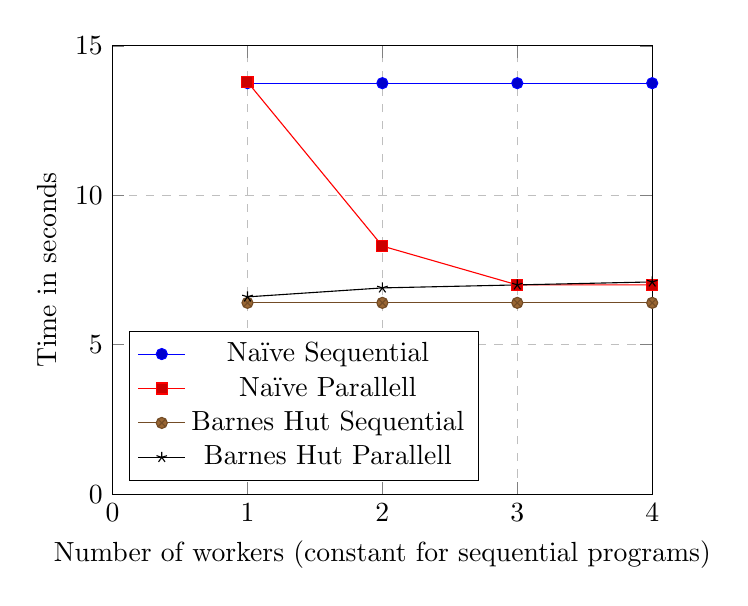
\begin{tikzpicture}
\begin{axis}[
  ylabel={Time in seconds},
  xlabel={Number of workers (constant for sequential programs)},
  xmin=0, xmax=4,
  ymin=0, ymax=15,
  legend pos=south west,
  ymajorgrids=true,
  xmajorgrids=true,
  grid style=dashed,
  legend entries={Na\"{i}ve Sequential, Na\"{i}ve Parallell, Barnes Hut Sequential,
  Barnes Hut Parallell}
]
\addplot coordinates {(1,13.75)(2,13.75)(3,13.75)(4,13.75)};
\addplot coordinates {(1,13.79)(2,8.3)(3,7.0)(4,7.0)};
\addplot coordinates {(1,6.4)(2,6.4)(3,6.4)(4,6.4)};
\addplot coordinates {(1,6.6)(2,6.9)(3,7.0)(4,7.1)};
\end{axis}
\end{tikzpicture}
\end{center}

\caption{Performance with 120 particles}
\label{fig:120}
\end{figure}

\begin{table}
\begin{center}
\begin{tabular}{| l | l | l | l | l |}
\hline
Name & Workers & $t(120)$ & $t(180)$ & $t(240)$\\ \hline
Na\"{i}ve Sequential & N/A & 13.76 & 30.85 & 54.81\\ \hline
Na\"{i}ve Parallell & 1 & 13.79 & 30.91 & 54.97\\ \hline
Na\"{i}ve Parallell & 2 & 8.3 & 16.68 & 29.19\\ \hline
Na\"{i}ve Parallell & 3 & 7.0 & 12.51 & 27.99\\ \hline
Na\"{i}ve Parallell & 4 & 7.0 & 10.29 & 18.67\\ \hline
Barnes-Hut Sequential & N/A & 6.4 & 10.45 & 15.22\\ \hline
Barnes-Hut Parallell & 1 & 6.6 & 10.76 & 15.74 \\ \hline
Barnes-Hut Parallell & 2 & 6.9 & 10.58 & 14.89 \\ \hline
Barnes-Hut Parallell & 3 & 7.0 & 9.13 & 13.70\\ \hline
Barnes-Hut Parallell & 4 & 7.1 & 9.93 & 13.24\\ \hline
\end{tabular}
\end{center}
\caption {$t(n)$ s performance with $n$ particles over 50 000 time steps}
\label{tab:120}
\end{table}

\begin{table}
\begin{center}
\begin{tabular}{| l | l | l | l | l |}
\hline
Name & Workers & $t(2000)$\\ \hline
Na\"{i}ve Sequential & N/A & 51.29 \\ \hline
Na\"{i}ve Parallell & 1 & 51.29 \\ \hline
Na\"{i}ve Parallell & 4 & 24.47 \\ \hline
Barnes-Hut Sequential & N/A & 3.94 \\ \hline
Barnes-Hut Parallell & 1 & 4.34  \\ \hline
Barnes-Hut Parallell & 4 & 2.96\\ \hline
\end{tabular}
\end{center}
\caption {$t(n)$ s performance with $n$ particles over 2000 time steps}
\label{tab:2000}
\end{table}

\begin{figure}
\begin{center}
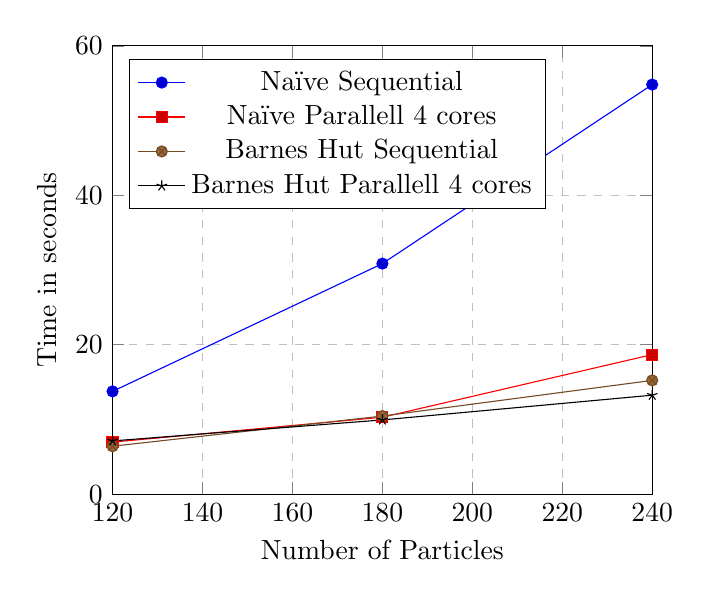
\begin{tikzpicture}
\begin{axis}[
  ylabel={Time in seconds},
  xlabel={Number of Particles},
  xmin=120, xmax=240,
  ymin=0, ymax=60,
  legend pos=north west,
  ymajorgrids=true,
  xmajorgrids=true,
  grid style=dashed,
  legend entries={Na\"{i}ve Sequential, Na\"{i}ve Parallell 4 cores, Barnes Hut Sequential,
  Barnes Hut Parallell 4 cores}
]
\addplot coordinates {(120,13.75)(180,30.85)(240,54.81)};
\addplot coordinates {(120,6.96)(180,10.29)(240,18.67)};
\addplot coordinates {(120,6.41)(180,10.45)(240,15.22)};
\addplot coordinates {(120,7.12)(180,9.93)(240,13.24)};
\end{axis}
\end{tikzpicture}
\end{center}

\caption{Performance Development with more Particles}
\label{fig:devparticles}
\end{figure}

\newpage
\begin{appendices}
\section{Performance.py Time Results}
\lstinputlisting{time}

\section{Common Listings for all applications}
\lstinputlisting{../gravn_common.c}

\newpage
\section{Listings for section \ref{subsec:seq_sq}}
\lstinputlisting{../seq_sq.c}

\newpage
\section{Listings for section \ref{subsec:par_sq}}
\lstinputlisting{../par_sq.c}

\section{Listings for section \ref{subsec:seq_nlg}}
\lstinputlisting{../seq_nlg.c}

\newpage
\section{Listings for section \ref{subsec:par_nlg}}
\lstinputlisting{../par_nlg.c}

\newpage
\section{Broken parallellization of \ref{subsec:par_nlg}}
\label{sec:par_nlg.broken}
\lstinputlisting{par_nlg.diff}

\newpage
\section{Listings for help script plot.py}
\label{sec:plotpy}
\lstinputlisting[language=Python]{../plot.py}

\newpage
\section{Listings for help script performance.py}
\label{sec:perfpy}
\lstinputlisting[language=Python]{../performance.py}

\newpage
\section{Listings for Makefile}
\lstinputlisting{../Makefile}
\end{appendices}

\end{document}

